\chapter{Dynamic 3D Object Insertion}\label{chp:ObjectLoading}

In order to realize the insertion of a 3D object from a CAD file, a plug-in with this functionality was developed simply called CADRuntimeImporter(CRI). Alongside it a standalone Unreal prototype project, named CADRuntimePresenter(CRP), was made that incorporates CRI in order to demonstrate how it can be used for a multi-user desktop and VR environment. The whole mechanism can be split into three major sections: opening and parsing the files, generating the objects and lastly user interaction with said objects. How all of that was implemented and what sort of advantages and disadvantages these approaches have, will be discussed in this chapter.
%%%%%%%%%%%%%%%%%%%%%%%%%%%%%%%%%%%%%%%%%%%%%%%%%%%%%%%%%%%%%%%%%%%%%%%%%%%%%%%%%%%%%%%%%%%%%%%%%%%%%%%%
\section{Loading and Parsing CAD Files}

The first step in creating an object in runtime is naturally opening the desired file and getting the required data from it in runtime as well. As Unreal Engine is written in C++, it is not surprising that opening up a file isn't too much of an issue. What makes this simpler is the fact that Unreal also offers this in their FileHelper class with the functions LoadFileToString() and LoadFileToArray(). The first function can load a text file into a string, while the other loads binary files into an array of bytes. This is only directly available in C++ and therefore had to be exposed to Blueprints. As this functionality is more of a utility, it isn't the best idea to attach it to a specific object. Luckily for such purposes Unreal offers Blueprint Function Libraries. This is just a special type of Unreal C++ class in which only static functions can be defined. These functions then become available to be used in any Blueprint without needing any instanced objects.\\

Something that is slightly more complicated is actually choosing the file. Here Unreal does technically offer the ability to open a file dialog but this is strictly a developer only module and can't be used in finished products. Even neglecting that, it wouldn't work in VR so a separate solution would have been needed anyway. Due to this a file picker in CRPs UI had to be written. The end result of that can be seen in Figure \ref{fig:FilePicker}. The design is rather simple but offers all the necessary functionality, especially that it is compatible with VR and only displays supported file formats.\\

\begin{figure}[htpb]
	\centering
	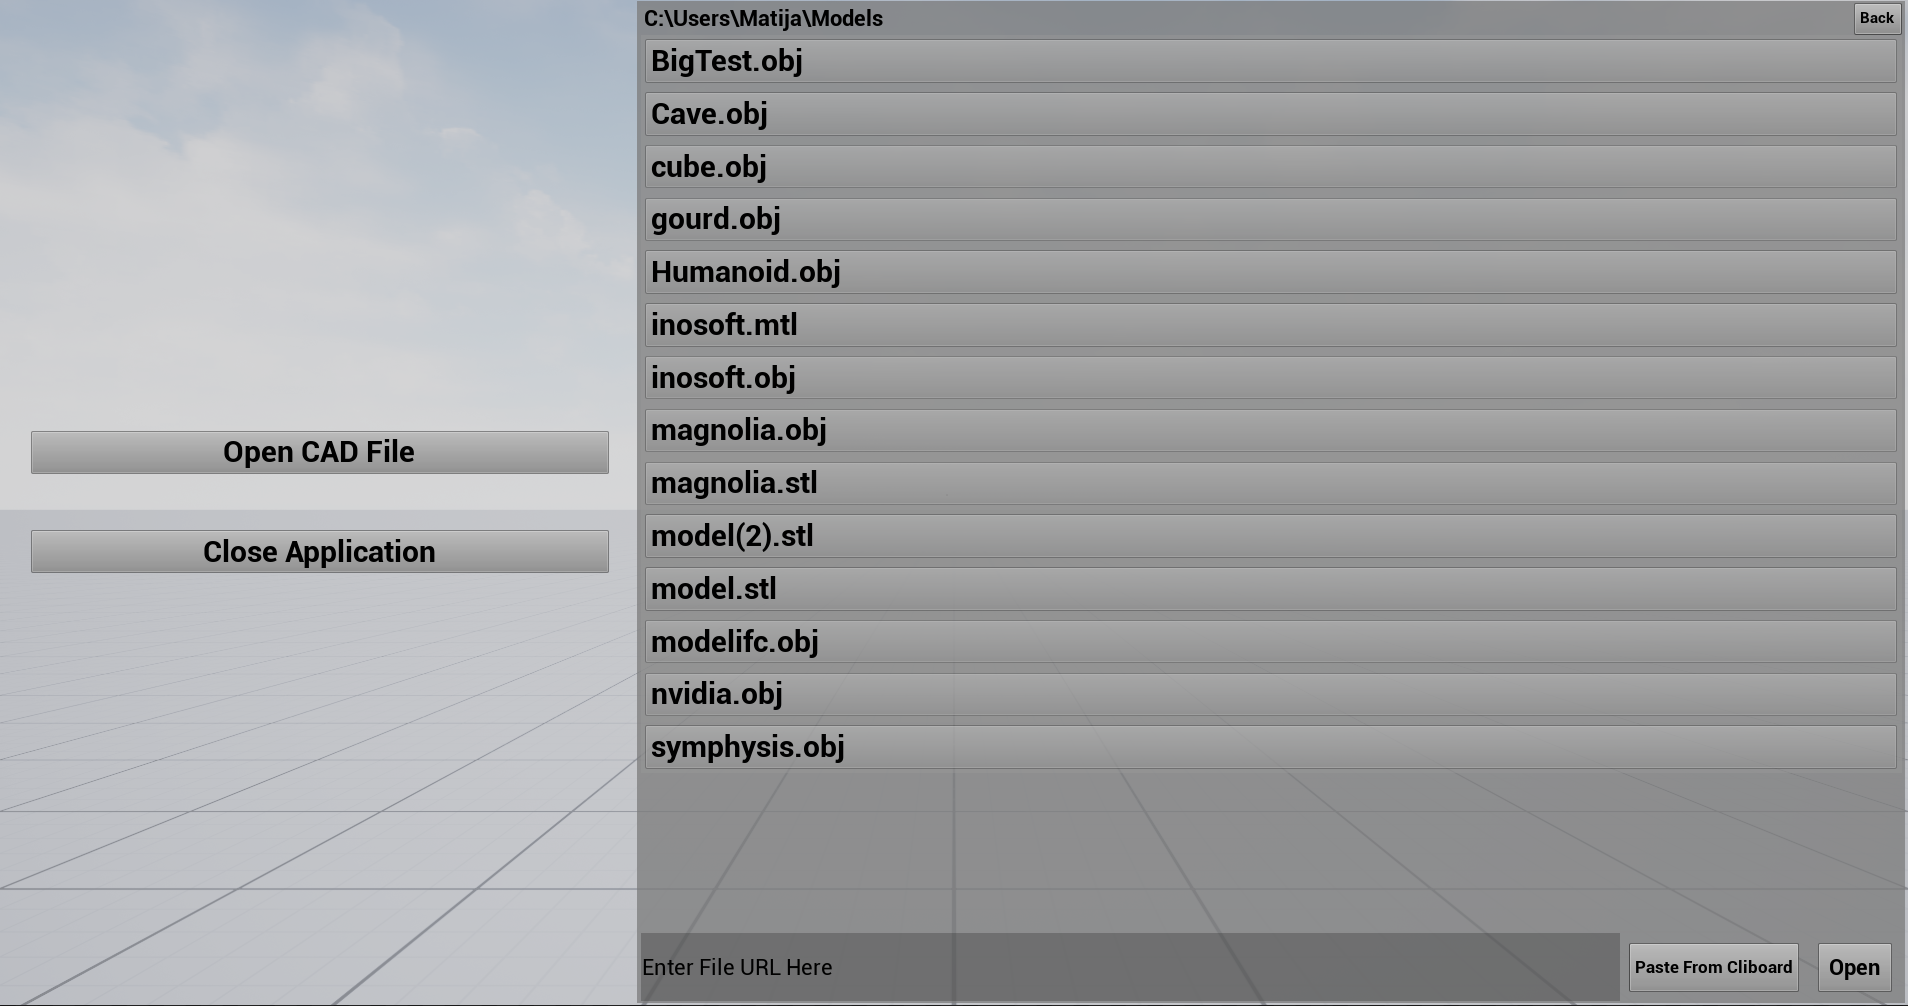
\includegraphics[width=0.9\textwidth]{fig/FilePicker2.png}
	\caption[CAD Runtime Presenter File Picker]{File Picker for CRP\protect}
	\label{fig:FilePicker}
\end{figure}

For a single user this would be enough, they could choose a file and then it could be parsed for object generating. Complications arise once there are multiple users involved. If a user were to open a file in such a scenario, the object would appear only in the world of that user and not for other users or even on the server. This could cause many issues since the clients world would not match servers, which is the authoritative instance. The problem lies in the fact that the new object needs to be created on every client and on the server. In order for that to happen every machine needs access to the required data, not just the client who has the file available on their machine.

\subsection{Wavefront OBJ and STL}


%%%%%%%%%%%%%%%%%%%%%%%%%%%%%%%%%%%%%%%%%%%%%%%%%%%%%%%%%%%%%%%%%%%%%%%%%%%%%%%%%%%%%%%%%%%%%%%%%%%%%%%%%%%%%%%%%%%%%%%%%
\section{Runtime Mesh Generation}
\subsection{Runtime Mesh Component}
\subsection{Material Generation}
\section{Object Interaction}\label{chp:ObjectInteraction}

\subsection{Mouse and Keyboard}

\subsection{Virtual Reality}



